\documentclass[11pt]{article}

\usepackage{amsmath, amssymb, amsthm}
\usepackage{tikz}

\theoremstyle{plain}
\newtheorem{thm}{Theorem}[section]
\newtheorem*{thm*}{Theorem}
\newtheorem{prop}[thm]{Proposition}
\newtheorem{lem}[thm]{Lemma}
\newtheorem*{lem*}{Lemma}
\newtheorem{dfn}[thm]{Definition}
\newtheorem{cor}[thm]{Corollary}
\newtheorem{claim}[thm]{Claim}
\newtheorem{conj}[thm]{Conjecture}
\newtheorem{ques}[thm]{Question}
\newtheorem*{rem}{Remark}


\oddsidemargin  0pt
\evensidemargin 0pt
\marginparwidth 40pt
\marginparsep 10pt
\topmargin 0pt
\headsep 10pt
\textheight 8.2in
\textwidth 6.4in
\renewcommand{\baselinestretch}{1.1}

\newcommand{\codeg}{\text{codeg}}
\newcommand{\BBE}{\mathbb{E}}
\newcommand{\BFP}{\mathbf{P}}
\usepackage{amsmath}
\usepackage{amsthm}
\usepackage{amssymb}
\usepackage{mathtools}
\usepackage{hyperref}
\usepackage{url}





\usepackage{graphicx}
\usepackage{caption}
\usepackage{subcaption}

\def\eQb#1\eQe{\begin{eqnarray*}#1\end{eqnarray*}}
\def\eQnb#1\eQne{\begin{eqnarray}#1\end{eqnarray}}
\providecommand{\e}[1]{\ensuremath{\times 10^{#1}}}
\providecommand{\pb}[0]{\pagebreak}
\DeclarePairedDelimiter\ceil{\lceil}{\rceil}
\DeclarePairedDelimiter\floor{\lfloor}{\rfloor}

\newcommand{\E}{\mathrm{E}}
\newcommand{\Var}{\mathrm{Var}}
\newcommand{\Cov}{\mathrm{Cov}}

\def\Qb#1\Qe{\begin{question}#1\end{question}}
\def\Sb#1\Se{\begin{solution}#1\end{solution}}


\newtheoremstyle{quest}{\topsep}{\topsep}{}{}{\bfseries}{}{ }{\thmname{#1}\thmnote{ #3}.}
\theoremstyle{quest}
\newtheorem*{definition}{Definition}
\newtheorem*{theorem}{Theorem}
\newtheorem*{lemma}{Lemma}
\newtheorem*{question}{Question}
\newtheorem*{preposition}{Preposition}
\newtheorem*{exercise}{Exercise}
\newtheorem*{challengeproblem}{Challenge Problem}
\newtheorem*{solution}{Solution}
\newtheorem*{remark}{Remark}
\usepackage{verbatimbox}
\usepackage{listings}
\usepackage{mathrsfs}
\date{}
\title{\vspace{-0.7cm}
Number Theory : Problem Set I}

\author{
Youngduck Choi 
\thanks{Department of Mathematics, Courant Institute of Mathematical Sciences, 
yc1104@nyu.edu; If you find an error and want to share with me, 
you can reach me via email.
}}

\begin{document}

\maketitle

\begin{abstract}
This work contains solutions to some exercises in the problem set I.
\end{abstract}


\begin{question}[1-1]
\hfill
\begin{figure}[h!]
  \centering
    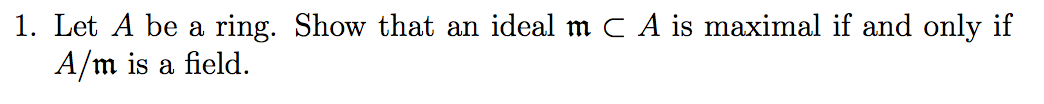
\includegraphics[width=0.7\textwidth]{ANT-s1-p1.png}
\end{figure}
\end{question}
\begin{solution} \hfill \\
By proposition 1.1 in Atiyah-MacDonald, there is a one-to-one correspondence between
the ideals of $\mathfrak{b}$ of $A$, which contains $\mathfrak{m}$, and the 
ideals $\bar{\mathfrak{b}}$ of $A / \mathfrak{m}$. Now, by proposition 1.2 in 
Atiyah-MacDonald, $A / \mathfrak{m}$ is a field iff the only ideals of $
A / \mathfrak{m}$ are $(0)$ and $(1)$, and by the one-to-one correspondence,
the later is equivalent to $\mathfrak{m}$ and $A$ being the only ideals
containing $\mathfrak{m}$, which is precisely definition of $\mathfrak{m}$
being maximal. \hfill $\qed$
 
\end{solution}

\newpage

\begin{question}[1-2]
\hfill
\begin{figure}[h!]
  \centering
    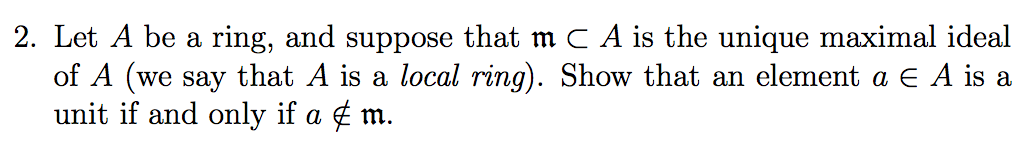
\includegraphics[width=0.7\textwidth]{ANT-s1-p2.png}
\end{figure}
\end{question}
\begin{solution} \hfill \\
Suppose $a \in A$ is a unit. Then, there exists $b \in A$, such that 
$ab = 1$. If $a \in \mathfrak{m}$, then $1 \in \mathfrak{m}$, and $\mathfrak{m} = A$,
which contradicts the fact that $\mathfrak{m}$ is maximal, hence. Therefore,
\eQb
a \>\>\> \text{is a unit} &\implies& a \not\in \mathfrak{m}.
\eQe
From Atiyah-MacDonald, Corollary 1.5, which uses 
a standard Zorn's lemma argument, we know that every non-unit of $A$ is 
contained in a maximal ideal. Therefore, by the uniqueness of $\mathfrak{m}$
as a maximal ideal, 
\eQb
a \>\>\> \text{is a non-unit} &\implies& a \in \mathfrak{m},
\eQe
and hence, by contrapositive,
\eQb
a \not \in \mathfrak{m} &\implies& a \>\>\> \text{is a unit},
\eQe
which concludes
\eQb
a \not \in \mathfrak{m} &\iff& a \>\>\> \text{is a unit},
\eQe
as required. \hfill $\qed$


\end{solution}

\newpage

\begin{question}[1-3]
\hfill
\begin{figure}[h!]
  \centering
    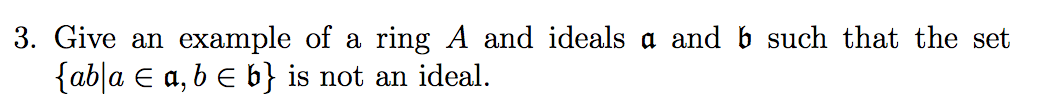
\includegraphics[width=0.7\textwidth]{ANT-s1-p3.png}
\end{figure}
\end{question}
\begin{solution} \hfill \\
Consider $A = \mathbb{R}[x,y]$, and $\mathfrak{a} = \mathfrak{b} = (x,y)$. 
Then, $x^2 , y^2 \in \{ab : a \in \mathfrak{a}, b \in \mathfrak{b}\}$, 
but $x^2 + y^2 \not\in \{ab : a \in \mathfrak{a}, b \in \mathfrak{b} \}$.  \hfill 
$\qed$ 
\end{solution}

\newpage

\begin{question}[1-4]
\hfill
\begin{figure}[h!]
  \centering
    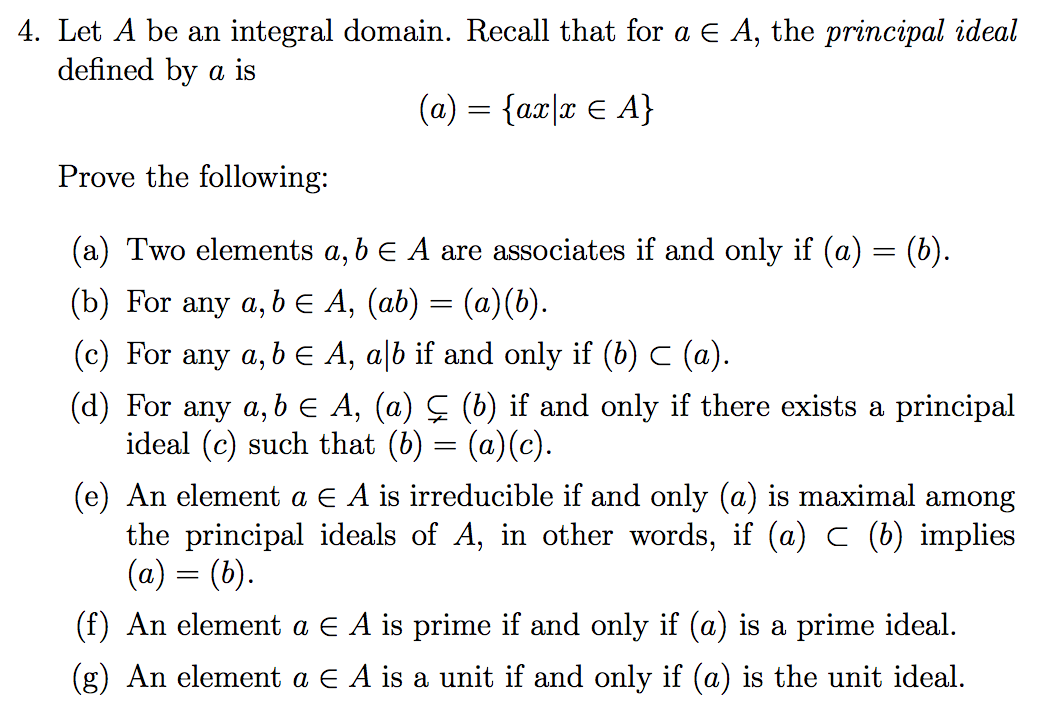
\includegraphics[width=0.7\textwidth]{ANT-s1-p4.png}
\end{figure}
\end{question}
\begin{solution} \hfill \\
\textbf{(a)} Observe that $a,b \in A$ are associates, there exists a unit $c$ such that
$a = bc$ is equivalent to there exists $c,d$ units such that $a = bc$  and $b = ad$.
To see this, if $c$ is a unit and $a = bc$, then there exists $d$ such that $cd = 1$,
and multiplying both sides by $d$ gives, $ad = b$, and by definition $d$ is a unit.

\smallskip

\noindent Suppose $a,b$ are associates. Then, if $ax \in (a)$, then set $y = cx$,
so $ax = bcx - by \in (b)$. Therefore, $(a) \subset (b)$ and similarly, by the
above discussion $(b) \subset (a)$ and hence $(a) = (b)$. Conversely, suppose
that $(a) = (b)$. Then, $a = bx$ for some $x \in A$, and $b = ay$ for some $y \in A$.
Therefore, $a = ayx$, so $1 = yx$. This shows that $x$ is a unit, and $a,b$
are associates. 

\bigskip

\noindent \textbf{(b)} We wish to show
\eQb
(ab) &=& \{ abx \> | \> x \in A\} = \{ax \> | \> x \in A\} \{ bx \> | \> x \in A\}
= (a)(b). 
\eQe 
For any $x \in A$, $abx = (ab)x$, so it is clear that 
\eQb
(ab) \subset (a)(b).
\eQe
Now, for $axby$ for any $x,y \in A$, $axby = abxy$ so 
\eQb
(a)(b) \subset (ab),
\eQe
which completes the proof.

\bigskip 

\noindent \textbf{(c)} Suppose $(b) \subset (a)$. Then, for any $x \in A$,
$bx = ay$ for some $y \in A$, and as $A$ is an integral domain, $b = ayx^{-1}$, so
$a|b$. Now, if $a|b$ then, by definition, $b = ay$ for some $y \in A$. Then,
for any $x \in A$, $bx = ayx$, so $(b) \subset (a)$, and we are done.

\bigskip

\noindent \textbf{(d)} Suppose $(a)$ is not contained in $(b)$. Then, there exists
$e \in A$, such that for all $y \in A$, $ae \neq by$.

\bigskip

\noindent \textbf{(e)} We have the following sequence of equivalence: 
\eQb
a \>\>\> \text{is irreducible} &\iff& \forall b,x \in A, \exists y \in A \> .s.t 
\>\> bx = ay \\ 
&\iff& \forall b \in A,  (b) \subset (a).
\eQe

\bigskip

\noindent \textbf{(f)} We have the following sequence of equivalence:
\eQb
(a) \>\>\> \text{is prime} &\iff& \forall b,c \in A, (bc = az \>\>\> \text{for some}
z \in A \implies a|b \>\>\> \text{or} \>\>\> a|c) \\
&\iff& a \>\>\> \text{is prime}.
\eQe

\bigskip

\noindent \textbf{(g)} We have the following sequence of equivalence:
\eQb
a \>\>\> \text{is unit} &\iff& \text{there exists} \>\>\> b \in A \>\> s.t. \>\> ab = 1 \\
&\iff& 1 \in (a) \iff (a) \>\>\> \text{is unit ideal}, 
\eQe
which completes the proof. \hfill $\qed$

\end{solution}

\newpage

\begin{question}[1-5]
\hfill
\begin{figure}[h!]
  \centering
    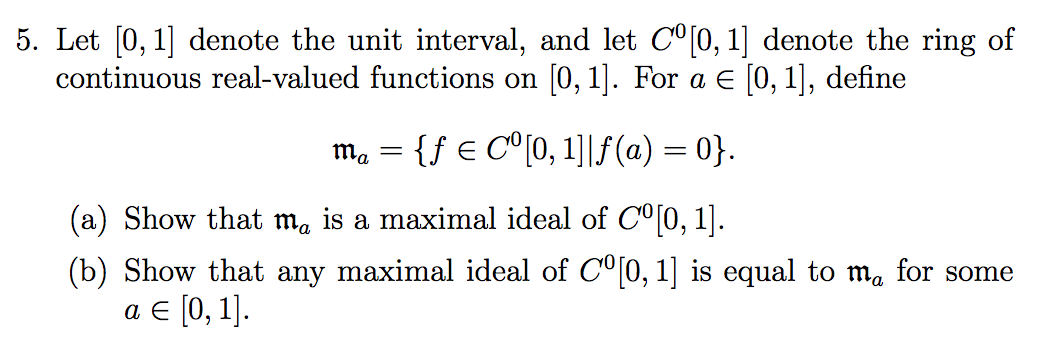
\includegraphics[width=0.7\textwidth]{ANT-s1-p5.png}
\end{figure}
\end{question}
\begin{solution} \hfill \\
We prove the statements in a slightly more general setting. Let $X$ be compact 
and Hausdorff space, and $C(X)$ be the ring of all real-valued continuous functions
on $X$. For each $x \in X$, let $\mathfrak{m}_x$ be the set of all $f \in C(X)$ such
that $f(x) = 0$.  

\bigskip

\noindent 
\textbf{(a)} Now, for any $x \in X$, we know that $\text{eval}_x:C(X) \to \mathbb{R}$,
defined by 
\eQb
\text{eval}_x(f) &\mapsto& f(x) \>\>\>\>\> (f \in C(X))
\eQe
is a surjective ring-homomorphism. Then, $\mathfrak{m}_x$ can be viewed as a kernel
of $\text{eval}_x$, so $\mathfrak{m}_x$ is maximal.  

\bigskip

\noindent
\textbf{(b)} Now, with (a) established, we can view $x \mapsto \mathfrak{m}_x$ 
as a map from $X$ to $\text{Max}(C(X))$, where the later denotes the set of
all maximal ideals of $C(X)$. We denote this map as $\mu$. Then, $(b)$ asserts
that $\mu$ is surjective, which we show now. Let $\mathfrak{m}$ be any
maximal idea in $C(X)$. Set
\eQb
V = \{ x \in X \> : \> f(x) = 0 \>\>\> \text{for all} \>\>\> f \in \mathfrak{m} \}.
\eQe 
Suppose $V$ is empty. Then, for each $x \in X$, we can find $f_x \in \mathfrak{m}$
such that $f_x(x) \neq 0$. By continuity of $\{f_x\}_{x in X}$, we can choose
an open cover of $X$,
$\{U_x\}_{x \in X}$, such that $f_x(U_x) \cap \{ 0\} = \emptyset$ for all $x \in X$.
Now, by compactness, there exists a sub-cover of the cover $\{U_i\}_{i \leq n}$.
Now, set 
\eQb
f = \sum_{i \leq n} f_i^2,
\eQe
where $f_i$s are the corresponding functions in $\mathfrak{m}$ for $U_i$s in
the construction. Then, $f \in \mathfrak{m}$ 
does not vanish anywhere, so it is a unit, which contradicts
the fact that $\mathfrak{m}$ is a maximal ideal. Hence, $V$ is non-empty, so $x_0 \in
V$ for some $x_0 \in X$. Then, $\mathfrak{m} \subset \mathfrak{m}_{x_0}$, and by 
maximality of $\mathfrak{m}$ and $\mathfrak{m}_{x_0}$, 
we see that $\mathfrak{m} = \mathfrak{m}_{x_0}$. In other words, $\mathfrak{m} = 
\mu(x_0)$. Therefore, $\mu$ is surjective and, we are done. \hfill $\qed$
 
 

\end{solution}


\end{document}
